\documentclass[aspectratio=169,xcolor={dvipsnames,table}]{beamer}
\usepackage[no-math,deluxe,haranoaji]{luatexja-preset}
\renewcommand{\kanjifamilydefault}{\gtdefault}
\renewcommand{\emph}[1]{{\upshape\bfseries #1}}
\usetheme{metropolis}
\setbeamertemplate{blocks}[rounded][shadow=false]
\metroset{block=fill}
%%%%%%%%%%%%%%%%%%%%%%%%%%
\setbeamertemplate{navigation symbols}{}
\usecolortheme[rgb={0.7,0.2,0.2}]{structure}
%%%%%%%%%%%%%%%%%%%%%%%%%%
%% Change alert block colors
%%% 1- Block title (background and text)
\setbeamercolor{block title alerted}{fg=mDarkTeal, bg=mLightBrown!45!yellow!45}
\setbeamercolor{block title example}{fg=magenta!10!black, bg=mLightGreen!70}
%%% 2- Block body (background)
\setbeamercolor{block body alerted}{bg=mLightBrown!25}
\setbeamercolor{block body example}{bg=mLightGreen!15}
%%%%%%%%%%%%%%%%%%%%%%%%%%%
%%%%%%%%%%%%%%%%%%%%%%%%%%%
%% さまざまなアイコン
%%%%%%%%%%%%%%%%%%%%%%%%%%%
%\usepackage{fontawesome}
\usepackage{fontawesome5}
\usepackage{figchild}
\usepackage{twemojis}
\usepackage{utfsym}
\usepackage{bclogo}
\usepackage{marvosym}
\usepackage{fontmfizz}
\usepackage{pifont}
\usepackage{phaistos}
\usepackage{worldflags}
\usepackage{jigsaw}
\usepackage{tikzlings}
\usepackage{tikzducks}
\usepackage{scsnowman}
\usepackage{epsdice}
\usepackage{halloweenmath}
\usepackage{svrsymbols}
\usepackage{countriesofeurope}
\usepackage{tipa}
\usepackage{manfnt}
%%%%%%%%%%%%%%%%%%%%%%%%%%%
\usepackage{tikz}
\usetikzlibrary{calc,patterns,decorations.pathmorphing,backgrounds}
\usepackage{tcolorbox}
\usepackage{tikzpeople}
\usepackage{circledsteps}
\usepackage{xcolor}
\usepackage{amsmath}
\usepackage{booktabs}
\usepackage{chronology}
\usepackage{signchart}
%%%%%%%%%%%%%%%%%%%%%%%%%%%
%% 場合分け
%%%%%%%%%%%%%%%%%%%%%%%%%%%
\usepackage{cases}
%%%%%%%%%%%%%%%%%%%%%%%%%%
\usepackage{pdfpages}
%%%%%%%%%%%%%%%%%%%%%%%%%%%
%% 音声リンク表示
\newcommand{\myaudio}[1]{\href{#1}{\faVolumeUp}}
%%%%%%%%%%%%%%%%%%%%%%%%%%
%% \myAnch{<名前>}{<色>}{<テキスト>}
%% 指定のテキストを指定の色の四角枠で囲み, 指定の名前をもつTikZの
%% ノードとして出力する. 図には remember picture 属性を付けている
%% ので外部から参照可能である.
\newcommand*{\myAnch}[3]{%
  \tikz[remember picture,baseline=(#1.base)]
    \node[draw,rectangle,line width=1pt,#2] (#1) {\normalcolor #3};
}
%%%%%%%%%%%%%%%%%%%%%%%%%%
%% \myEmph コマンドの定義
%%%%%%%%%%%%%%%%%%%%%%%%%%
%\newcommand{\myEmph}[3]{%
%    \textbf<#1>{\color<#1>{#2}{#3}}%
%}
\usepackage{xparse} % xparseパッケージの読み込み
\NewDocumentCommand{\myEmph}{O{} m m}{%
    \def\argOne{#1}%
    \ifx\argOne\empty
        \textbf{\color{#2}{#3}}% オプション引数が省略された場合
    \else
        \textbf<#1>{\color<#1>{#2}{#3}}% オプション引数が指定された場合
    \fi
}
%%%%%%%%%%%%%%%%%%%%%%%%%%%
%%%%%%%%%%%%%%%%%%%%%%%%%%%
%% 文末の上昇イントネーション記号 \myRisingPitch
%% 通常のイントネーション \myDownwardPitch
%% https://note.com/dan_oyama/n/n8be58e8797b2
%%%%%%%%%%%%%%%%%%%%%%%%%%%
\newcommand{\myRisingPitch}{
\begin{tikzpicture}[scale=0.3,baseline=0.3]
\draw[->,>=stealth] (0,0) to[bend right=45] (1,1);
\end{tikzpicture}
}
\newcommand{\myDownwardPitch}{
\begin{tikzpicture}[scale=0.3,baseline=0.3]
\draw[->,>=stealth] (0,1) to[bend left=45] (1,0);
\end{tikzpicture}
}
%%%%%%%%%%%%%%%%%%%%%%%%%%%%
%\AtBeginSection[%
%]{%
%  \begin{frame}[plain]\frametitle{授業の流れ}
%     \tableofcontents[currentsection]
%   \end{frame}%
%}

\usetikzlibrary{tikzmark}
%%%%%%%%%%%%%%%%%%%%%%%%%%%
\title{English is fun.}
\subtitle{be動詞---am, are, is---}
\author{}
\institute[]{}
\date[]

%%%%%%%%%%%%%%%%%%%%%%%%%%%%
%% TEXT
%%%%%%%%%%%%%%%%%%%%%%%%%%%%
\begin{document}
%%%%%%%%%%%%%%%%%%%%%%%%%%%%
%\begin{frame}[label=waiting]{}
%%%%%%\phantomsection\label{section}
%\thispagestyle{empty}
%\Large
%\raggedright
%
%予定の時刻になったらはじまります
%
%\vfill
%
%\raggedleft
%
%The lesson will begin at the scheduled time.
%\end{frame}
%%%%%%%%%%%%%%%%%%%%%%%%%%%%%%
\begin{frame}[label=title]
%\phantomsection\label{section-1}
\thispagestyle{empty}
\titlepage
\end{frame}
%%%%%%%%%%%%%%%%%%%%%%%%%%%%%%%%%%%%%%%%%%%%%%%%%%
\section*{授業の流れ}
\begin{frame}[plain]
  \frametitle{授業の流れ}
  \tableofcontents
\end{frame}
%%%%%%%%%%%%%%%%%%%%%%%%%%%%%%%
%\section{復習--主語と動詞--}

%\begin{frame}[plain]{復習}
%
%\Large
%
%主語と動詞
% \begin{exampleblock}{Topics for Today}
%\begin{itemize}
% \item   英文の骨格は主語と動詞です
% \item   英語は語順がだいじです
% \item   英文にはかならず主語が必要
%\end{itemize}
%     \end{exampleblock}
%
%\end{frame}
%%%%%%%%%%%%%%%%%%%%%%%%%%%%%%%%
%\begin{frame}[plain]\frametitle{Exercises}
%日本語を参考にして、主語と動詞を指摘してください。
%\begin{enumerate}
%    \item \alt<2->{\Circled[outer color=Maroon]{You}}{You} \alt<3->{\Circled[outer color=NavyBlue]{have}}{have} a nice car. あなたはいい車を持っている。
% \item \alt<4->{\Circled[outer color=Maroon]{I}}{I} \alt<5->{\Circled[outer color=NavyBlue]{play}}{play} the piano. わたしはピアノを弾きます。
%    \item \alt<6->{\Circled[outer color=Maroon]{They}}{They} \alt<7->{\Circled[outer color=NavyBlue]{watch}}{watch} TV. 彼らはテレビを見ます。
%    \item \alt<8->{\Circled[outer color=Maroon]{We}}{We} \alt<9->{\Circled[outer color=NavyBlue]{study}}{study} English. わたしたちは英語を勉強します。
% \item \alt<10->{\Circled[outer color=Maroon]{I}}{I} \alt<11->{\Circled[outer color=NavyBlue]{write}}{write} a letter. わたしは手紙を書きます。
%     \item \alt<12->{\Circled[outer color=Maroon]{Birds}}{Birds} \alt<13->{\Circled[outer color=NavyBlue]{sing}}{sing}. 鳥は歌います。
%    \item \alt<14->{\Circled[outer color=Maroon]{Dogs}}{Dogs} \alt<15->{\Circled[outer color=NavyBlue]{swim}}{swim} well. 犬はじょうずに泳ぎます。
%     \item \alt<16->{\Circled[outer color=Maroon]{They}}{They} \alt<17->{\Circled[outer color=NavyBlue]{like}}{like} music. 彼らは音楽が好きです。
%\end{enumerate}
%
%% Embed the sound file
%\onslide<1->{%
%\myaudio{./audio/003_sv_03.mp3}
%}
%\end{frame}

%%%%%%%%%%%%%%%%%%%%%%%%%%%%%%%%
\section{be動詞とは}
\begin{frame}[plain,label=what_is_be]\frametitle{be動詞とは}
 % \setbeamercovered{transparent}
  \begin{enumerate}
   \item<1-> I \textbf<14-20>{\color<14-20>{Maroon}{am}} a student. \onslide*<2>{わたしは生徒です。}\onslide*<14-20>{(I $=$ a student)}\hfill\onslide*<21-26>{\footnotesize  student: 生徒、学生\hspace{6pt}cf. study}
   \item<1-> You \textbf<15-20>{\color<15-20>{Maroon}{are}} my friend. \onslide*<4>{あなたはわたしのともだちです。}\onslide*<15-20>{(You $=$ my friend)}\hfill\onslide*<22-26>{\footnotesize  my: わたしの friend \textipa{/fr\'end/} ともだち}
   \item<1-> He \textbf<16-20>{\color<16-20>{Maroon}{is}} tall. \onslide*<6>{彼は背が高い。}\onslide*<16-20>{(He $=$ tall)}\hfill\onslide*<23-26>{\footnotesize  tall: 背が高い}
   \item<1-> She \textbf<17-20>{\color<17-20>{Maroon}{is}} kind. \onslide*<8>{彼女は親切だ。}\onslide*<17-20>{(She $=$ kind)}\hfill\onslide*<24-26>{\footnotesize  kind: 親切な、優しい}
   \item<1-> The sky \textbf<18-20>{\color<18-20>{Maroon}{is}} blue. \onslide*<10>{空は青い。}\onslide*<18-20>{(The sky $=$ blue)}\hfill\onslide*<25-26>{\footnotesize  the sky: 空 blue: 青い}
   \item<1-> They \textbf<19-20>{\color<19-20>{Maroon}{are}} my classmates. \onslide*<12>{彼らはわたしのクラスメートです。}\onslide*<19-20>{(They $=$ my classmates)}\hfill\onslide*<26>{\footnotesize  classmate: クラスメート、級友}
  \end{enumerate}

\bigskip

\begin{block}<20->{Topics for Today}\small
\begin{itemize}\setbeamertemplate{items}[square]
 \item \textbf{am, are, is}
\begin{itemize}\setbeamertemplate{items}[circle]
 \item まとめて\,\Circled[fill color=white]{\,be動詞\,}\,といいます
 \item イコール($=$)の意味
\end{itemize}
\end{itemize}
\end{block}

% Embed the sound file
\hfill{\tiny 0251}\,{\scriptsize \myaudio{audio/002_be_01.mp3}}
\end{frame}
%%%%%%%%%%%%%%%%%%%%%%%%%%%%%%%%%%%%%%%%%%%%%%%%%%%
\begin{frame}[plain]\frametitle{am, are, is --- みんな、なかまです}
 \centering
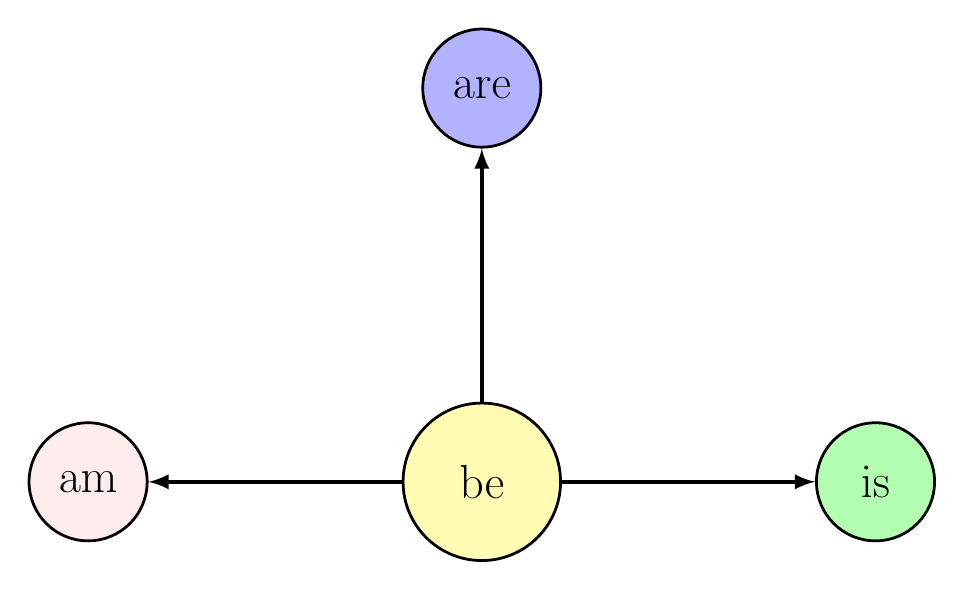
\begin{tikzpicture}
% 補助グリッドを描画
%\draw[step=1cm, gray!20, very thin] (-6,-2) grid (6,6);
% ノードの定義と配置
\visible<1->{\node[circle, draw=black, fill=pink!30,minimum size=15mm, line width=1pt] (B) at (-5,0) {\LARGE am};}
\visible<2->{\node[circle, draw=black, fill=blue!30, minimum size=15mm, line width=1pt] (C) at (0,5) {\LARGE are};}
\visible<3->{\node[circle, draw=black, fill=green!30, minimum size=15mm, line width=1pt] (D) at (5,0) {\LARGE is};}
\visible<4->{\node[circle, draw=black, fill=yellow!30, minimum size=20mm, line width=1pt] (A) at (0,0) {\LARGE be};}
% ノード間の線の描画
\visible<5->{\draw[-latex, line width=1.5pt] (A) -- node[above] {} (B);}
\visible<5->{\draw[-latex, line width=1.5pt] (A) -- node[sloped, above] {} node[sloped, below] {} (C);}
\visible<5->{\draw[-latex, line width=1.5pt] (A) -- node[above] {} (D);}
\end{tikzpicture}
\end{frame}
%%%%%%%%%%%%%%%%%%%%%%
\begin{frame}[plain]{be動詞、どれ使う?}
 \centering\Large

be動詞$\left\{\begin{tabular}[c]{l}
       am\\are\\is\end{tabular}\right\}$の使い分けを学習しよう
\end{frame}
%%%%%%%%%%%%%%%%%%%%%%%%%%%%%%%%%%%%%%%%%%%%%
\section{I am 〜}
\begin{frame}<1->[plain,label=i_am]\frametitle{I am 〜.}
%\begin{frame}<1-20>[plain,label=i_am]\frametitle{I am 〜.}
 % \setbeamercovered{transparent}
  \begin{enumerate}
   \item<1-> \textbf{\color{Maroon}{I am}} a student. \onslide*<2>{わたしは生徒です。}\hfill\onslide*<15-20>{\footnotesize  student: 生徒、学生}
   \item<1-> \textbf{\color{Maroon}{I am}} tall. \onslide*<4>{わたしは背が高い。}\hfill\onslide*<16-20>{\footnotesize  tall: 背が高い}
   \item<1-> \textbf{\color{Maroon}{I am}} 13 years old. \onslide*<6>{わたしは13歳です。}\hfill\onslide*<17-20>{\footnotesize  〜 years old: 〜歳だ (〜には数字がはいります)}
   \item<1-> \textbf{\color{Maroon}{I am}} John. \onslide*<8>{わたしはジョンです。}
   \item<1-> \textbf{\color{Maroon}{I am}} happy. \onslide*<10>{わたしは幸せです。}\hfill\onslide*<18-20>{\footnotesize  happy: 幸せだ}
   \item<1-> \textbf{\color{Maroon}{I am}} from Tokyo. \onslide*<12>{わたしは東京の出身です。}\hfill\onslide*<19-20>{\footnotesize  from 〜: 〜の出身だ}
  \end{enumerate}

\bigskip

\begin{block}<14->{Topics for Today}\small
\begin{itemize}\setbeamertemplate{items}[square]
 \item 主語がIのときbe動詞は\textbf{am}をつかいます
 \item \textbf{I am} 〜.をひとつのパターンとして覚えよう
\end{itemize}
     \end{block}

% Embed the sound file
\hfill{\tiny 0250}\,{\scriptsize \myaudio{./audio/002_be_02.mp3}}


\end{frame}
%%%%%%%%%%%%%%%%%%%%%%%%%%%%%%%%%%%%
\begin{frame}[plain,t]{Exercises}

\begin{tcolorbox}[colframe=black,
  colback=Yellow!10!white,
  colbacktitle=Yellow!40!white,
  coltitle=black, %fonttitle=\bfseries,
  title=自己紹介]
John Smithさんは、
Boston出身で年齢は12歳です。

John Smithさんになったつもりで自己紹介文を作成してみよう。
\end{tcolorbox}


\bigskip

\begin{enumerate}
 \item わたしはJohn Smithです。
 \item わたしは〜の出身です。\hfill{}from 〜
 \item わたしは〜歳です。\hfill{}〜 years old
\end{enumerate}

\end{frame}
%%%%%%%%%%%%%%%%%%%%%%%%%%%%%%%%%%%%%%%%%%%%%%%%%%
\section*{Coffee Break}
%%%%%%%%%%%%%%%%%%%%%%%%%%%%%%%%%%%%%%%%%%%%%%%%%
\begin{frame}[plain]{Boston}

\raggedleft

\includegraphics[height=.9\textheight]{./images/boston_1.jpg}

\vspace*{-8pt}
\tiny

``Boston'' by jeffgunn is licensed under CC BY 2.0. \\
To view a copy of this license, visit \url{https://creativecommons.org/licenses/by/2.0/?ref=openverse}.
  \end{frame}
%%%%%%%%%%%%%%%%%%%%%%%%%%%%%%%%%%%%%%%%%%%%%%%%%%
\begin{frame}[plain]{Boston}

\raggedleft

\includegraphics[height=.9\textheight]{./images/boston_2.jpg}

\vspace*{-8pt}
\tiny


``Boston \`{a} l'heure bleue'' by Manu\_H is licensed under CC BY 2.0.\\
To view a copy of this license, visit \url{https://creativecommons.org/licenses/by/2.0/?ref=openverse}.

 \end{frame}
%%%%%%%%%%%%%%%%%%%%%%%%%%%%%%%%%%%%%%%%%%%%%%%%%%
\begin{frame}[plain]{Boston}

\raggedleft

\includegraphics[height=.9\textheight]{./images/boston_3.jpg}

\vspace*{-8pt}
\tiny

``Boston Rapid Transit Map'' by michaelvit is licensed under CC BY 2.0.\\
 To view a copy of this license, visit \url{https://creativecommons.org/licenses/by/2.0/?ref=openverse}.
 \end{frame}

%%%%%%%%%%%%%%%%%%%%%%%%%%%%%%%%%%%%%
\begin{frame}[plain,label=im]{Answer}
 \Large

\begin{enumerate}
 \item \visible<1->{I am}\onslide*<4->{($=$I'm)} \visible<1->{John Smith.}
 \item \visible<2->{I am}\onslide*<4->{($=$I'm)} \visible<2->{from Boston.}
 \item \visible<3->{I am}\onslide*<4->{($=$I'm)} \visible<3->{twelve years old.}
\end{enumerate}

\normalsize
{\tiny 0137}\,{\scriptsize \myaudio{audio/002_be_021.mp3}}
\hfill{}%
{\tiny 0136}\,{\scriptsize \myaudio{audio/002_be_022.mp3}}


\normalsize
\begin{block}<5->{Topics for Today}\small
\setbeamercovered{transparent}
\begin{itemize}\setbeamertemplate{items}[square]
 \item  主語がIのときbe動詞は\textbf{am}をつかいます
 \item  \textbf{I am} 〜.をひとつのパターンとして覚えよう
 \item<6-> \textbf{I am $=$ I'm}\tikzmark{target1}\\
\mbox{}\hfill{}\tikzmark{pointer1}%
\visible<7->{{\scriptsize 短縮形といいます。 \Circled[fill color=white]{~'~}\,をapostrophy\,(アポストロフィ)といいます\phantom{あ}}}
\end{itemize}
     \end{block}


\begin{tikzpicture}[remember picture,overlay]
 \visible<7->{\draw[<-,opacity=.4,line width=2pt] ([yshift=-2pt]pic cs:target1) to[out=-15, in=180] ([xshift=-2pt, yshift=2pt] pic cs:pointer1);}
\end{tikzpicture}
\end{frame}

%%%%%%%%%%%%%%%%%%%%%%%%%%%%%%%%%%%%%%%%%%%
\section{You are 〜}
\begin{frame}[plain,label=youare,t]\frametitle{You are 〜.}
 % \setbeamercovered{transparent}
  \begin{enumerate}
   \item<1-> \textbf{\color{Maroon}{You are}} my friend. \visible<2->{{\scriptsize あなたはわたしのともだちです。}}\hfill\visible<1->{\scriptsize  friend \textipa{/fr\'end/} ともだち、友人}
   \item<1-> \textbf{\color{Maroon}{You are}} very kind. \visible<3->{{\scriptsize あなたはとても親切だ。}}\hfill\visible<1->{\scriptsize  kind \textipa{/k\'aInd/} 親切だ}
   \item<1-> \textbf{\color{Maroon}{You are}} a good student. \visible<4->{{\scriptsize あなたはいい生徒です。}}\hfill\visible<1->{\scriptsize  student: 生徒}
   \item<1-> \textbf{\color{Maroon}{You are}} good at baseball. \visible<5->{{\scriptsize あなたは野球がうまい。}}\hfill\visible<1->{\scriptsize  good at 〜がうまい、得意だ}
   \item<1-> \textbf{\color{Maroon}{You are}} busy. \visible<6->{{\scriptsize あなたは忙しい。}}\hfill\visible<1->{\scriptsize  busy \textipa{/b\'Izi/} 忙しい}
   \item<1-> \textbf{\color{Maroon}{You are}} from Chiba. \visible<7->{{\scriptsize あなたは千葉の出身です。}}\hfill\visible<1->{\scriptsize  from 〜の出身だ}
  \end{enumerate}

\vfill

\begin{block}<8->{Topics for Today}\small
\begin{itemize}\setbeamertemplate{items}[square]
 \item 主語がyouのときbe動詞は\textbf{are}をつかいます
 \item \textbf{You are} 〜.をひとつのパターンとして覚えよう
\end{itemize}
     \end{block}

% Embed the sound file
\hfill{\tiny 0245}\,{\scriptsize \myaudio{audio/002_be_03.mp3}}

\end{frame}
%%%%%%%%%%%%%%%%%%%%%%%%%%%%%%%%%%%%%%%%%%%%%%%%%
\begin{frame}<1-9>[plain]{Exercises}

{\small あたえられた日本語の意味になるよう(~~~~~~)に適当な1語を補いましょう}

\begin{enumerate}
 \item {\small あなたは親切だ}。(\alt<1>{~~\phantom{You}~~}{~~\textcolor{Maroon}{You}~~})~~are kind.
 \item {\small あなたは背が高い。}You~~(\alt<1-2>{~~\phantom{are}~~}{~~\textcolor{Maroon}{are}~~})~~tall.
 \item {\small あなたは親切だ。}(\alt<1-4>{~~\phantom{You're}~~}{~~\textcolor{Maroon}{You're}~~})~~kind.
 \item {\small あなたは背が高い。}(\alt<1-5>{~~\phantom{You're}~~}{~~\textcolor{Maroon}{You're}~~})~~tall.
\end{enumerate}

\vfill

 \begin{block}<4->{Topics for Today}\small
\setbeamercovered{transparent}
\begin{itemize}\setbeamertemplate{items}[square]
 \item<4,9> 主語がyouのときbe動詞は\textbf{are}をつかいます
 \item<4,9> \textbf{You are} 〜.をひとつのパターンとして覚えよう
 \item<7-> \textbf{You are} $=$ \textbf{You're}\tikzmark{target2} \\
\mbox{}\hfill{}\visible<8->{{\scriptsize \tikzmark{pointer2}短縮形といいます。 \Circled[fill color=white]{~'~}\,をapostrophy\,(アポストロフィ)といいます\phantom{あ}}}
\end{itemize}
     \end{block}

% Embed the sound file
\hfill{\tiny 0158}\,{\scriptsize \myaudio{audio/002_be_031.mp3}}


\begin{tikzpicture}[remember picture,overlay]
 \visible<8->{\draw[<-,opacity=.4,line width=2pt] ([yshift=-2pt]pic cs:target2) to[out=-15, in=180] ([xshift=-2pt, yshift=2pt] pic cs:pointer2);}
\end{tikzpicture}


\end{frame}
%%%%%%%%%%%%%%%%%%%%%%%%%%%%%%%%%%%%%%%%%%%%
%\againframe{waiting}
%\againframe{title}
%%%%%%%%%%%%%%%%%%%%%%%%%%%%%%%%%%%%%%%%%%%
%%%%%%%%%%%%%%%%%%%%%%%%%%%%%
% 背景色を黒に変更
%\setbeamercolor{background canvas}{bg=black}
%\begin{frame}
%\centering
%  \textcolor{white}{\Huge\bfseries The Fourth of July}\pause
%
% \vspace{30pt}
%
%  \textcolor{white}{\Huge\bfseries Independence Day}
%
%\end{frame}
%\setbeamercolor{background canvas}{bg=}
%%%%%%%%%%%%%%%%%%%%%%%%%%%%%%%
%
%{
%  \usebackgroundtemplate{\includegraphics[width=\paperwidth,height=\paperheight]{./images/betsy_ross_flag.png}}
%  \begin{frame}
%    %\frametitle{Slide 3 with background image}
%    %Content of slide 3.
%  \end{frame}
%}
%%%%%%%%%%%%%%%%%%%%%%%%%%%%%%%%%%%
\section{I am, You are以外の場合(1)}
\begin{frame}[plain,label=recap_1]\frametitle{I am, You are以外の場合(1)}
 % \setbeamercovered{transparent}
  \begin{enumerate}
   \item<1-> This \textbf{\color{Maroon}{is}} my pencil. \onslide*<2->{{\scriptsize これはわたしの鉛筆です。}}\hfill\onslide*<1->{\scriptsize this: これ cf. that:あれ pencil: 鉛筆}
   \item<1-> He \textbf{\color{Maroon}{is}} my classmate. \onslide*<3->{{\scriptsize 彼はわたしのクラスメートです。}}\hfill\onslide*<1->{\scriptsize classmate: クラスメート、級友}
   \item<1-> She \textbf{\color{Maroon}{is}} a good singer. \onslide*<4->{{\scriptsize 彼女は歌がうまい。}}\hfill\onslide*<1->{\scriptsize singer: 歌い手、歌手}
   \item<1-> Your bike \textbf{\color{Maroon}{is}} new. \onslide*<5->{{\scriptsize あなたの自転車は新しい。}}\hfill\onslide*<1->{\scriptsize  bike: 自転車 new: 新しい}
   \item<1-> George \textbf{\color{Maroon}{is}} busy. \onslide*<6->{{\scriptsize ジョージは忙しい。}}\hfill\onslide*<1->{\scriptsize  busy: 忙しい}
   \item<1-> Jane \textbf{\color{Maroon}{is}} from France. \onslide*<7->{{\scriptsize ジェーンはフランスの出身です。}}\hfill\onslide*<1->{\scriptsize from  〜の出身だ France: フランス}
  \end{enumerate}

\vfill

\begin{block}<8->{主語がIまたはYou以外のとき1}\small
主語が単数のときはisを使います
\begin{itemize}\setbeamertemplate{items}[square]
 \item 1つ It, This, That, The book \ldots{} 
 \item 1人 He, She, Jane, My father \ldots{} 
\end{itemize}  
     \end{block}

% Embed the sound file
\hfill{\tiny 0248}\,{\scriptsize \myaudio{audio/002_be_04.mp3}}

\end{frame}
%%%%%%%%%%%%%%%%%%%%%%%%%%%%%%%
\begin{frame}<1-6>[plain]{Exercises}

 {\small つぎの各2文が同じ意味になるよう空所に適当な語を補いましょう}

\begin{enumerate}
 \item \begin{enumerate}
	\item She is very kind.
	\item \alt<1>{(~~\phantom{She's}~~)}{(~~\textcolor{BurntOrange}{\bfseries She's}~~)}\,\,very kind.
       \end{enumerate}
 \item \begin{enumerate}
	\item He is from Australia.\hfill\scalebox{2.2}{\twemoji{globe showing Asia-Australia}}\,\,\scalebox{.4}{\worldflag{AU}}
	\item \alt<1-2>{(~~\phantom{He's}~~)}{(~~\textcolor{BurntOrange}{\bfseries He's}~~)}\,\,from Australia.
       \end{enumerate}
 \item \begin{enumerate}
	\item It is a great movie.\hfill\scalebox{2.2}{\twemoji{film projector}}
	\item \alt<1-3>{(~~\phantom{It's}~~)}{(~~\textcolor{BurntOrange}{\bfseries It's}~~)}\,\,a great movie.
       \end{enumerate}
 \item \begin{enumerate}
	\item That is her new car.\hfill\scalebox{2}{\faCar}
	\item \alt<1-4>{(~~\phantom{That's}~~)}{(~~\textcolor{BurntOrange}{\bfseries That's}~~)}\,\,her new car.
       \end{enumerate}
\end{enumerate}

\begin{block}<6->{短縮形}
\begin{itemize}\setbeamertemplate{items}[square]
 \item He is\,($=\text{He's}$)\,\,\,\,/\,\,\,She is\,($=\text{She's}$)\,\,\,\,/\,\,\,It is\,($=\text{It's}$)\,\,\,\,/\,\,\,That is\,($=\text{That's}$)
\end{itemize}  
     \end{block}

\vspace*{-5pt}
% Embed the sound file

\hfill{\tiny 0200}\,{\scriptsize \myaudio{audio/002_be_041.mp3}}\\
\hfill{\scriptsize それぞれ2行目の短縮形の練習です}

\end{frame}

\section{I am, You are以外の場合(2)}

\begin{frame}[plain]\frametitle{I am, You are以外の場合(2)}
 % \setbeamercovered{transparent}
  \begin{enumerate}
   \item<1-> These \textbf{\color{Maroon}{are}} my pencils. \onslide*<2->{{\scriptsize これらはわたしの鉛筆です。}}\hfill\onslide*<1->{\scriptsize these: これら cf. those: あれら}
   \item<1-> They \textbf{\color{Maroon}{are}} my classmates. \onslide*<3->{{\scriptsize 彼らはわたしのクラスメートです。}}\hfill\onslide*<1->{\scriptsize they: 彼ら}
   \item<1-> They \textbf{\color{Maroon}{are}} kind. \onslide*<4->{{\scriptsize 彼らは親切だ。}}\hfill\onslide*<1->{\scriptsize kind: 親切な}
   \item<1-> The flowers \textbf{\color{Maroon}{are}} beautiful. \onslide*<5->{{\scriptsize その花は美しい。}}\hfill\onslide*<1->{\scriptsize flower: 花 beautiful: 美しい}
   \item<1-> We \textbf{\color{Maroon}{are}} busy. \onslide*<6->{{\scriptsize わたしたちは忙しい。}}\hfill\onslide*<1->{\scriptsize we: わたしたち busy: 忙しい}
   \item<1-> Jane and George \textbf{\color{Maroon}{are}} from France. \onslide*<7->{{\scriptsize ジェーンとジョージはフランス出身だ。}}\hfill\onslide*<1->{\scriptsize from 〜の出身だ}
  \end{enumerate}

\bigskip

\begin{block}<8->{主語がIまたはYou以外のとき2}\small
主語が複数のときは are を使います
\begin{itemize}\setbeamertemplate{items}[square]\small
 \item 2つ以上 they, these, those, flowers \ldots
 \item 2人以上 we, they, Peter and Mary \ldots
\end{itemize}
     \end{block}

% Embed the sound file

\hfill{\tiny 0248}\,{\scriptsize \myaudio{audio/002_be_05.mp3}}

\end{frame}
%%%%%%%%%%%%%%%%%%%%%%%%%%%%%
%\section{まとめ}
%\begin{frame}[plain]{復習}
%
%\begin{block}{areのまとめ}
%\begin{itemize}
% \item   I, You 以外で複数(2つ以上)のモノや人が主語のとき\,\,---\,主語が複数のとき\,---\,\,はareを使います
%%% \item We are\,($=\text{We're}$)\,\,\,\,/\,\,\,They are\,($=\text{They're}$)
%\end{itemize}  
%     \end{block}
%\end{frame}
%%%%%%%%%%%%%%%%%%%%%%%%%%%%%%%%%%%%%
\begin{frame}<1-4>[plain]{Exercises}

 {\small つぎの各2文が同じ意味になるよう空所に適当な語を補いましょう}

\begin{enumerate}
 \item \begin{enumerate}
	\item We are best friends.
	\item \alt<1>{(~~\phantom{We're}~~)}{(~~\textcolor{BurntOrange}{\bfseries We're}~~)}\,\,best friends
       \end{enumerate}
 \item \begin{enumerate}
	\item They are from Italy.
	\item \alt<1-2>{(~~\phantom{They're}~~)}{(~~\textcolor{BurntOrange}{\bfseries They're}~~)}\,\,from Italy        \end{enumerate}
\end{enumerate}

\vfill

\begin{block}<4->{Topic for Today ---短縮形---}
\begin{itemize}\setbeamertemplate{items}[square]
 \item We are\,($=\text{We're}$)\,\,\,\,/\,\,\,They are\,($=\text{They're}$)
\end{itemize}
     \end{block}

% Embed the sound file

\hfill{\tiny 0135}\,{\scriptsize \myaudio{audio/002_be_051.mp3}}\\
\hfill{\scriptsize それぞれ2行目の短縮形の練習です}

\end{frame}
%%%%%%%%%%%%%%%%%%%%%%%%%%%%%%%%%%%%%%%%%%%%%%%%%%%
%%%%%%%%%%%%%%%%%%%%%%
%\begin{frame}[plain]{areを使う場合}
%
%\begin{block}{areのまとめ}
%\begin{itemize}\setbeamertemplate{items}[square]
% \item   I, You 以外で複数(2つ以上)のモノや人が主語のとき\,\,---\,主語が複数のとき\,---\,\,はareを使います
% \item We are\,($=\text{We're}$)\,\,\,\,/\,\,\,They are\,($=\text{They're}$)
%\end{itemize}  
%     \end{block}
%
%
%\end{frame}
%%%%%%%%%%%%%%%%%%%%%%%%%%%%%%%%%%
\section{be動詞のまとめ}
\begin{frame}[plain]\frametitle{まとめ}

be動詞---am, are, is---は主語に応じて使い分けがあります

\bigskip

\begin{block}{be動詞の使い分け}

{\large
\begin{numcases}{\text{ }}
 \text{\mbox{}\,\,{}Iが主語}&$\longrightarrow$\,\,\,\,\,\,{}\text{am}\\
 \text{\mbox{}\,\,{}Youが主語}&$\longrightarrow$\,\,\,\,\,\,{}\text{are}\\[5pt]
 \text{{\scriptsize I, You以外が主語のとき}}\\
 \text{\mbox{}\,\,{}単数(1つ、1人)}&$\longrightarrow$\,\,\,\,\,\,{}\text{is}\tag{3--a}\\
 \text{\mbox{}\,\,{}複数(2つ、2人以上)}&$\longrightarrow$\,\,\,\,\,\,{}\text{are}\tag{3--b}
\end{numcases}
}
\end{block}
\end{frame}
%%%%%%%%%%%%%%%%%%%%%%%%%%%%%%%%%%%%%%%%%%
\begin{frame}[plain]\frametitle{be動詞}
 \centering
\begin{tikzpicture}
% 補助グリッドを描画
%\draw[step=1cm, gray!20, very thin] (-6,-2) grid (6,6);
% ノードの定義と配置
\visible<1->{\node[circle, draw=black, fill=yellow!30, minimum size=20mm, line width=1pt] (A) at (0,0) {\LARGE be動詞};}
\visible<2->{\node[circle, draw=black, fill=pink!30,minimum size=15mm, line width=1pt] (B) at (-6,0) {\LARGE am};}
\visible<3->{\node[circle, draw=black, fill=blue!30, minimum size=15mm, line width=1pt] (C) at (0,5) {\LARGE are};}
\visible<4->{\node[circle, draw=black, fill=green!30, minimum size=15mm, line width=1pt] (D) at (6,0) {\LARGE is};}

% ノード間の線の描画
\visible<5->{\draw[-latex, line width=1.5pt] (A) -- node[above] {主語がI} (B);}
%\visible<6->{\draw[-latex, line width=1.5pt] (A) -- node[sloped, above] {主語がYou}  node[sloped, below] {{\textcolor{Maroon}{主語が複数}}} (C);}
\visible<6->{\draw[-latex, line width=1.5pt] (A) -- node[sloped, above] {主語がYou}  node[sloped, below] {} (C);}
\visible<7->{\draw[-latex, line width=1.5pt] (A) -- node[sloped, above] {主語がYou}  node[sloped, below] {{\textcolor{Maroon}{主語が複数}}} (C);}
\visible<8->{\draw[-latex, line width=1.5pt] (A) -- node[above] {\textcolor{Maroon}{主語が単数}} node[below] {} (D);}
\end{tikzpicture}
\end{frame}
%%%%%%%%%%%%%%%%%%%%%%%%%%%%%%
%%%%%%%%%%%%%%%%%%%%%%%%%%%%%%%%%%%%%%%%%%
\begin{frame}[plain]{短縮形}
 \begin{center}
 \rowcolors{2}{NavyBlue!50}{yellow!40}
\begin{tabular}{ll}\toprule
{\small }&{\small 短縮形}\\\midrule
\visible<1->{I am}&\visible<2->{{\small I'm}}\\
\visible<1->{You are}&\visible<3->{{\small You're}}\\
\visible<1->{He is}&\visible<4->{{\small He's}}\\
\visible<1->{She is}&\visible<5->{{\small She's}}\\
\visible<1->{It is}&\visible<6->{{\small It's}}\\
\visible<1->{That is}&\visible<7->{{\small That's}}\\
\visible<1->{We are}&\visible<8->{{\small We're}}\\
\visible<1->{They are  }&\visible<9->{{\small They're  }}\\
\bottomrule
\end{tabular}%
\end{center}
\end{frame}
%%%%%%%%%%%%%%%%%%%%%%%%%%%%%%%%%%%%%%%
\begin{frame}[plain]{Exercises}
 
{\small 次の英文の(~~~~~~~~)内から動詞の正しい形を選び、○で囲みましょう}

\begin{enumerate}
 \item John~~( am / \alt<2->{\Circled[outer color=orange]{is}}{is} / are )~~a baseball player.
 \item You~~( \alt<3->{\Circled[outer color=orange]{are}}{are} / is / am )~~nice.
 \item This~~( am / \alt<4->{\Circled[outer color=orange]{is}}{is} / are )~~my cup.
 \item They~~( am / is / \alt<5->{\Circled[outer color=orange]{are}}{are} )~~my parents.
 \item We~~(am / \alt<6->{\Circled[outer color=orange]{are}}{are} / is )~~Japanese.
 \item I~~( \alt<7->{\Circled[outer color=orange]{am}}{am} / is / are )~~hungry.
\end{enumerate}

\mbox{}\hfill{\tiny 0239}\,{\scriptsize \myaudio{audio/002_be_06.mp3}}

\end{frame}
%%%%%%%%%%%%%%%%%%%%%%%%%%%%%%%%%


\end{document}


